\section{What look-ahead changes}
\label{sec:behaviour}

\begin{figure*}[t]
  \centering
  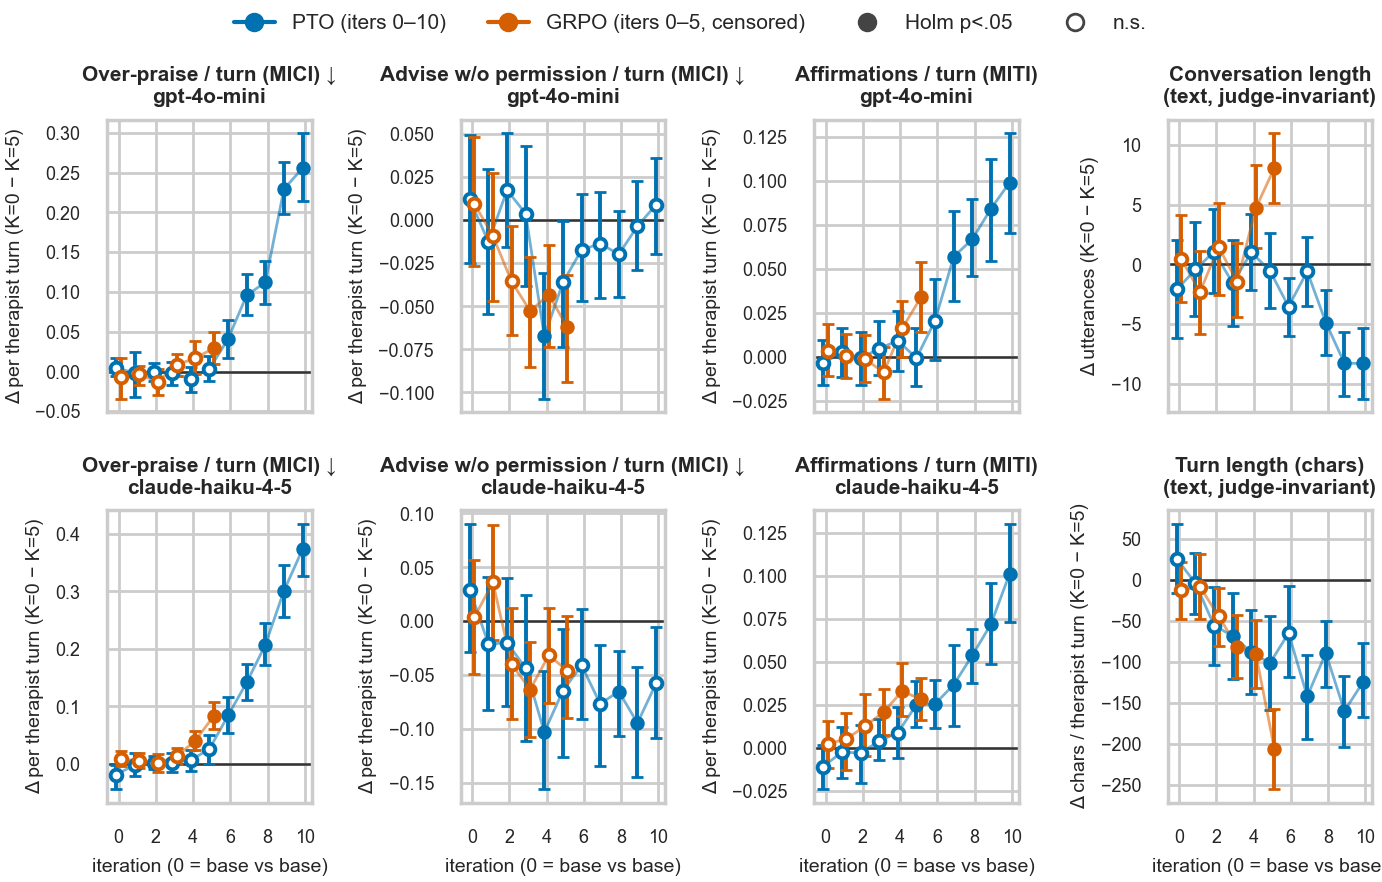
\includegraphics[width=0.96\textwidth]{figures/k_contrast_headline_fig_channels.png}
  \caption{Behaviour channels, persona-paired \Kz{}$-$\Kf{} by iteration ($n{=}96$; positive
    $=$ the \Kz{} policy does more of it). Rows: training oracle, held-out judge; right-hand
    column: grader-free text measures. Filled $=$ Holm-significant across iterations within a
    channel. GRPO \Kf{} is censored at iteration~5.}
  \label{fig:channels}
\end{figure*}

The reward contrasts of \S\ref{sec:reward} are small; the behavioural contrasts behind them are
not, and they are where the two optimizers agree.

\paragraph{Look-ahead closes the over-praise channel.} Under \Kz{} both optimizers end by
flattering. At PTO iteration~10 the \Kz{} policy over-praises $0.299$ times per therapist turn
against $0.043$ under \Kf{} (training oracle; $\Delta{=}{+}0.256$, $\dz{=}1.16$,
$p_{\text{Holm}}{<}10^{-3}$) and $0.448$ vs.\ $0.075$ under the held-out judge ($\dz{=}1.65$). GRPO shows the same sign at its
censored endpoint (iteration~5: $\dz{=}0.30$ oracle, $0.69$ held-out). By the endpoints
over-praise is $3.042/4.958{=}61\%$ (PTO, iteration~10) and $8.250/9.865{=}84\%$ (GRPO,
iteration~10) of the \Kz{} arms' MI-inconsistent acts per session under the training oracle
($56\%$ and $78\%$ under the held-out judge), against $19\%$ and $9\%$ for the \Kf{} arms (PTO
iteration~10; GRPO at its censored iteration~5, where the \Kz{} share is still $19\%$; $15\%$
and $6\%$ under the held-out judge; Figures~\ref{fig:channels} and~\ref{fig:composition}).

\paragraph{But the inconsistency is relocated, not removed.} Advice-without-permission runs the
other way, and it moves first: at PTO iteration~4 the \Kf{} policy already advises without
asking more often per turn ($\dz{=}{-}0.36$ on both graders, $p_{\text{Holm}}{=}.005$), whereas
the over-praise gap clears Holm only from iteration~7 (per session, training oracle; 6 under the
held-out judge). Table~\ref{tab:substitution} shows the consequence: for PTO every component of the trade keeps
its sign across the judge swap, but the per-session total keeps only its sign, not its
significance.

\begin{table}[t]
  \centering\footnotesize
  \setlength{\tabcolsep}{3pt}
  \begin{tabular}{@{}lrrrr@{}}
    \toprule
    & \multicolumn{2}{c}{oracle} & \multicolumn{2}{c}{held-out} \\
    \cmidrule(lr){2-3}\cmidrule(lr){4-5}
    \Kz{}$-$\Kf{} & $\Delta$ & \dz{} & $\Delta$ & \dz{} \\
    \midrule
    \multicolumn{5}{@{}l}{\emph{PTO, iter.\ 10 (\Kf{} 14.4 vs.\ \Kz{} 10.2 ther.\ turns)}} \\
    Over-praise / session       & $+2.42$ & $0.89^{*}$  & $+3.57$ & $1.00^{*}$ \\
    Advice w/o perm.\ / session & $-0.31$ & $-0.24$     & $-1.95$ & $-0.71^{*}$ \\
    Directing / session         & $-0.38$ & $-0.39^{*}$ & $-0.68$ & $-0.47^{*}$ \\
    All MI-incons.\ / session   & $+1.61$ & $0.45^{*}$  & $+0.53$ & $0.10$ \\
    All MI-incons.\ / turn      & $+0.23$ & $0.71^{*}$  & $+0.24$ & $0.66^{*}$ \\
    \midrule
    \multicolumn{5}{@{}l}{\emph{GRPO, iter.\ 5, censored (\Kf{} 11.3 vs.\ \Kz{} 15.3)}} \\
    Over-praise / session       & $+0.43$ & $0.38^{*}$  & $+1.25$ & $0.69^{*}$ \\
    Advice w/o perm.\ / session & $-0.03$ & $-0.02$     & $+1.04$ & $0.27$ \\
    All MI-incons.\ / session   & $+0.32$ & $0.13$      & $+1.89$ & $0.34^{*}$ \\
    All MI-incons.\ / turn      & $-0.06$ & $-0.24$     & $-0.02$ & $-0.05$ \\
    \bottomrule
  \end{tabular}
  \caption{The substitution at the matched endpoints, training oracle (\primaryjudge{}) and
    held-out judge (\heldoutjudge{}). Persona-paired \Kz{}$-$\Kf{}, $n{=}96$; positive $=$ the
    \Kz{} policy does more of it (all lower-is-better). ${}^{*}$ Holm $p<.05$ across iterations
    within a channel. The therapist-turn counts in the block headers are why per-session and
    per-turn totals disagree.}
  \label{tab:substitution}
\end{table}

\paragraph{The total is unit- and grader-specific.} Per therapist turn, MI-inconsistency at PTO
iteration~10 is lower under \Kf{} on both graders ($\dz{=}0.71$ oracle, $0.66$ held-out, both
$p_{\text{Holm}}{<}10^{-3}$). Per session it is lower only under the training oracle ($+1.61$
acts, $\dz{=}0.45$, $p_{\text{Holm}}{=}.001$; held-out $+0.53$, $\dz{=}0.10$,
$p_{\text{Holm}}{=}.84$), because the held-out judge counts the substituted advice at $1.95$
acts to the oracle's $0.31$. The denominator matters because \Kf{} PTO sessions are $8.3$
utterances longer, so a rate flatters the arm that talks longer; GRPO at iteration~5, with
shorter \Kf{} sessions, is the mirror image (per session lower under \Kf{} on the held-out
judge, $\dz{=}0.34$; per turn nominally higher, $\dz{=}{-}0.24$ oracle, n.s.). We therefore
report the substitution and not a reduction.

\paragraph{Session shape moves in opposite directions.} At PTO iteration~10 the \Kf{} sessions
run $28.7$ utterances to \Kz{}'s $20.4$ ($+8.3$ for \Kf{}; $|\dz|{=}0.55$,
$p_{\text{Holm}}{<}10^{-4}$); at GRPO iteration~5 they run $22.6$ to $30.7$ ($-8.1$,
$\dz{=}0.53$). Both \Kf{} arms write longer therapist turns ($+125$ chars for PTO,
$|\dz|{=}0.55$; $+207$ for GRPO, $0.81$). GRPO \Kz{} collapses to $0.32$ questions per turn by
iteration~5 ($0.15$ by 10) while GRPO \Kf{} holds $0.69$ ($|\dz|{=}0.61$,
$p_{\text{Holm}}{<}10^{-7}$); PTO shows no question-rate difference at iteration~10 ($0.55$ vs.\
$0.62$, n.s.; Figure~\ref{fig:shape}). \S\ref{sec:mechanism} traces the PTO lengthening to the
selection itself.

\paragraph{Held-out instruments: same alliance total, different alliance.} On WAI-SR, PTO \Kf{}
and \Kz{} tie on the total at iteration~10 (oracle $-0.04$, held-out $+0.10$, both n.s.), but
bond excess (Bond minus the Goal/Task mean) is higher under \Kz{} by $+0.22$ (oracle,
$\dz{=}0.43$) and $+0.27$ (held-out, $\dz{=}0.45$), both $p_{\text{Holm}}{=}.001$; GRPO shows the
same sign, weaker ($+0.15$ / $+0.13$, n.s.; Figure~\ref{fig:wai}). The
held-out judge's Q2 item profile says what the bond is made of: its late \Kz{} edge
(\S\ref{sec:reward}) sits on the emotional self-disclosure items 3 and 10 ($+1.10$ and $+1.03$
over \Kf{} at PTO iteration~10, $\dz{=}1.14$ / $1.00$, against $+0.27$ on the other fifteen);
the training oracle sees no item-level $K$ effect. Change-talk proportion (PCT)
rises under \Kf{} for GRPO on both graders (iteration~5: $-0.056$, $\dz{=}{-}0.31$; $-0.067$,
$\dz{=}{-}0.37$) and for PTO under the held-out judge only ($-0.051$, $\dz{=}{-}0.25$). Split by
scripted cooperation (32 personas each), the PCT gain and GRPO's reward gain (\QQ{}
$\dz{=}{-}0.56$ oracle, ${-}0.59$ held-out) sit in the Warms-up stratum; the Cooperative third
is at ceiling on the training oracle ($88$--$100\%$ of conversations $\geq 4.5$), so no $K$
contrast is observable there at the matched endpoints, and the held-out judge, which never reaches the ceiling, instead
credits \Kz{} PTO's warmth on those personas ($+0.57$, $\dz{=}0.77$; Figure~\ref{fig:hetero}).
